%%%%%%%%%%%%%%%%%%%%%%%%%%%%%%%%%%%%%%%%%%%%%%%%%%%%%%%%%%%%%%%%%%%%%%%%%%%%%%%
\documentclass[aps,pra,groupedaddress,12pt,
%               showpacs,%      display the PACS code(s)
               amsfonts,amssymb,
%                twocolumn,
               preprint
    ]{revtex4}
% ---------------------- load CTAN & macro packages ---------------------------
\usepackage{graphicx}
\usepackage{amsmath}
\usepackage{amssymb}
\usepackage{dcolumn}
\usepackage{revsymb}
\usepackage{natbib}
\usepackage{array}
\usepackage{xspace}
\usepackage{bm}
\usepackage{braket}
\usepackage{SE}  %       required style file containing macros for this paper

%%%%%%%%%%%%%%%%%%%%%%%%%%%%%%%%%%%%%%%%%%%%%%%%%%%%%%%%%%%%%%%%%%%%%%%%%%%%%%%
\begin{document}
%
\preprint{First Version: Aug 09, 2005; Final version: Nov 30, 2005}
\date{\today}
%
\title[Coupled Body-Frame Scattering Equations for Electron-Molecule Scattering]%
{Coupled Body-Frame Scattering Equations for Electron-Molecule Scattering}

\author{Hao \surname{Feng}}
\email[Electronic address: ]{ddsteed@163.com}
\affiliation{College of Physics, Sichuan University, Chengdu, Sichuan,
610065, P.R.China}

\begin{abstract}
  This note is modified from Prof.~Michael A.~Morrison's note in
  April 1977. The author derived all equations and augmented some proofs
  and corrected some errors.
\end{abstract}

\maketitle
\tableofcontents
% -----------------------------------------------------------------------------
\section{Equation for the Scattering Function}
The general (N-electron) molecule wavefunction cannot be separated as
the H$_2$ can, so we write the electronic wavefunction as
\begin{equation}
  \label{eq:ew}
  \ewt=\oneover{\sqrt{N!}}
  \sum_{\abp}\LC_{\abp}\sowa(1)\sowb(2)\cdots\sowp(N)
\end{equation}
where $\tau$ denotes the collection of target molecular electrons,
$\sowa(i)$ is the $\alpha^{th}$ single-particle spin orbital for
particle $i$, and $\LC_{\abp}$ is the Levi-Civita density\footnote{We
  sum over all possible values of $\alpha$, $\beta$, \ldots, $\pi$. So
  for N$_2$ with 14 molecular (spin) orbital, we have $\alpha$, $\beta$,
  $\gamma$, $\delta$, $\epsilon$, $\phi$ and each $\sum$ runs, e.g.,
  $\alpha$ = 1, 2, \ldots, 14. Lots of them!}
\begin{equation*}
  \LC_{\abp}=
  \begin{cases}
    0 &\text{if any 2 indices are equal} \\
    +1 &\text{even permutations} \\
    -1 &\text{odd permutations}
  \end{cases}
\end{equation*}
We use $\Ra$ to denote the nuclear coordinates (collectively). Since we
are in the Body-Fixed reference frame, $\nlg$ denote the electronic
state eigenfunction and its spin, respectively, for the $\gamma^{th}$
state of the target molecule. Thus $n$ collectively denotes symmetry
($\pm$) $g$ or $u$; and $\Lambda$, the projection of the total orbital
angular momentum (of the molecule) along $\hat{z}=\hat{R}$ ($\Sigma$,
$\Pi$, $\Delta$ for $\Lambda$ = 0, 1, 2, etc.). Now since we neglect
rotation, the ``remaining'' molecular wavefunction can be written as
(Born-Oppenheimer) \label{com:norot}
\begin{equation}
  \label{eq:mw}
  \mw_{\nlvg}(\tau;\Ra)=\ewt\vw_{\nlvg}^{vib}(\Ra)
\end{equation}
with $\vw_{\nlvg}^{vib}$ the vibrational wavefunction. Note that
$\ewn$ here depends on the spin coordinates of the target
electrons, $\sigma_1$, \ldots, $\sigma_N$. When we mean the
$\alpha^{th}$ spin orbital, we write $\sowa(i)$; the corresponding
spatial orbital is $\owa(\vri)$. Thus
\begin{equation}
  \label{eq:sw}
  \sowa(i) = \owa(\vri)\swa
\end{equation}
The full molecular wavefunction of \Eq{mw} satisfies the
Schr\"{o}dinger Equation
\begin{equation}
  \label{eq:mse}
  \Ham_{mol}\mw_{\nlvg}(\tau;\Ra) = E_{\nlvg}\mw_{\nlvg}(\tau;\Ra)
\end{equation}
where $\Ham_{mol}$ is the full non-relativistic molecular Hamiltonian,
written in general as
\begin{equation*}
  \Ham_{mol} = \Th + \sum_{\alpha\beta}\frac{\Za\Zb}{|\vRa-\vRb|}
              -\sum_{\alpha i}\frac{\Za}{|\vRa-\vri|}
              +\sum_{ij}\oneover{|\vri-\vrj|}
\end{equation*}

Now, the wavefunction for the system of electron $+$ molecule is
expanded as
\begin{equation}
  \label{eq:emw}
  \emw = \oneover{\sqrt{N+1}}\sum_{\gamma'}
         \sum_{i=1}^{N+1}(-1)^{N+1-i}\mwga\scf
\end{equation}
where $\scf$ is the scattering function including the spin dependence
\begin{equation}
  \label{eq:sfs}
  \scf=\sof\swg
\end{equation}
and the factor of $(N+1)^{-1/2}$ ensure consistent normalization with
\Eq{ew}. This function is anti-symmetric. For convenience, we shall
denote the target wavefunction as
\begin{equation}
  \label{eq:mwgb}
  \mwga = \mwgb
\end{equation}
where $\bar{i}$ denotes not including the $i^{th}$ electron.

Thus
\begin{equation}
  \label{eq:emwb}
  \emw = \oneover{\sqrt{N+1}}\sum_{\gamma'}
         \sum_{i=1}^{N+1}(-1)^{N+1-i}\mwgb\scf
\end{equation}
NOTE that for each $\gamma'$ we carry out the indicated $\sum_i$ ---
this summation is for purposes of antisymmetrizing and must be treated
carefully! Here $\gamma$ also labels the initial spin of the scattering
$e^-$. 

Our object is to determine an equation for the scattering function
$\sof$ such that $\emw$ satisfies the SE
\begin{equation}
  \label{eq:emse}
  (\Ham - E)\emw = 0
\end{equation}
where $E$, the total energy of the system, is related to the target
energy (for state $\gamma$) by
\begin{equation}
  \label{eq:eme}
  E = \oneover{2}k_\gamma{}^2 + E_{\nlvg}
\end{equation}

The full Hamiltonian is
\begin{equation}
  \label{eq:fham}
  \Ham = \Ham_{mol}(\tau;\Ra) + \Ther + \Vint(\vri,\ver;\Ra)
\end{equation}
where $\vri$ denotes all the spatial target electron coordinates, i.e.,
$\tau\equiv(\vri,\sigma_i)$. In general, the electron-molecule
interaction potential energy is (atomic units)
\begin{equation}
  \label{eq:vint}
  \Vint = -\sum_\alpha\frac{\Za}{|\ver-\vRa|} 
          +\sum_i\oneover{|\ver-\vri|}
\end{equation}

We shall eventually make the usual single-center expansion of the
(spatial) scattering function $\sof$, i.e.,
\begin{equation}
  \label{eq:sof}
  \sof = \oneover{r}\sum_{\elg\mg}\srf\sshf
\end{equation}
where the sum is over $\elg$ and $\mg$, of course.

Alright, the SE for the system becomes (from \Eq{emwb} and \Eq{emse})
\begin{equation}
  \label{eq:emsea}
  (\Ham - E)\oneover{\sqrt{N+1}}\sum_{\gamma'}\sum_i(-1)^{N+1-i}\mwgb\scf
\end{equation}
We now $\otimes$
\begin{equation*}
  \left[\mwgg\swgg\right]^*
\end{equation*}
and integrate over $\rd\tau\equiv \rd 1\cdots \rd N$ (includes sums over
the spin coordinates) and sum over $\sigma_{N+1}$\footnote{This is the
  most important step! Please learn this procedure.}. We also integrate
over $d\Ra$ (the vibrational coordinates), we get
\begin{equation}
  \label{eq:int1}
  \I =
  \matrixelement{\mwgg\swgg}
                {\Ham - E}
                {\sum_{\gamma'}\sum_i(-1)^{N+1-i}\mwgb\scf} = 0
\end{equation}

Before we begin churning way on the algebra for this, let's summarizing
the orthogonality relations we have to help us out:
\begin{enumerate}
\item We'll assure that the target wavefunctions, which satify \Eq{mse}
  have been normalized, 
  \begin{equation}
    \label{eq:otme}
    \matrixelementa{\mw_{\nlvg}}{\mw_{(\nlv)_{\gamma'}}}=
    \delta_{n_\gamma n_{\gamma'}}
    \delta_{\Lambda_\gamma\Lambda_{\gamma'}}
    \delta_{v_\gamma v_{\gamma'}}
  \end{equation}
\item For closed-shell targets, the PEP (Pauli Exclusive Principle)
  forbids the incident electron occupying a target orbital of the same
  symmetry, viz., for any scattering orbital, we have
  \begin{equation}
    \label{eq:otem}
    \matrixelementa{\sowa(i)}{\scf} = 0, \qquad \forall\alpha\in\gamma'
  \end{equation}
\end{enumerate}
It is easy (and useful!) to show the equivelence of \Eq{otem} to a more
general result, consider
\begin{equation}
  \label{eq:int2}
  \I_t\equiv\matrixelementa{\ew_{(\nl)_{\gamma'}}(\bar{i};\Ra)}{\scfj}_j,
  \qquad [\text{except} \quad i=j=N+1]
\end{equation}

Using \Eq{ew} for $\ew$, this integral becomes
\begin{align*}
  \I_t &=
  \oneover{\sqrt{N!}}\sum_{\abp}\LC_{\abp}
  \matrixelementa{\sowa(1)\sowb(2)\cdots\sowp(N)}{\scfj}_j \\
    &=\oneover{\sqrt{N!}}\sum_{\abp}\LC_{\abp}
      \sowa(1)\sowb(2)\cdots\sow_{\gamma-1}(j-1)\sow_{\gamma+1}(j+1)
      \cdots\sowp(N)\matrixelementa{\sow_\gamma(j)}{\scfj}_j 
\end{align*}
where $\sow_\gamma(j)$ is the spin-orbital corresponding to coordinates
$j$ in each term in the summation. But by \Eq{otem}, $\I_t=0$, so we have
for any $i$ (except $i=j=N+1$)
\begin{equation}
  \label{eq:otem2}
  \matrixelementa{\mw_{(\nlv)_{\gamma'}}(\bar{i};\Ra)}{\scfj}_j = 0,
  \qquad 1\leq j \leq N+1
\end{equation}
where we have combined $\I_t=0$ with \Eq{otem}. Notice that many
possibilities are covered by \Eq{otem2}. 

(From here on, we'll specialize to the case where no electronic
excitation is allowed. The treatment of orthogonality becomes somewhat
confusing if we allow for electronic excitation. And note that once we
use \Eq{otem2}, we are restricted bo closed shell
targets.\label{com:state}) 

Pulling the summation (now over $v_{\gamma'}$ only) outside of
\Eq{int1}, we have the integral
\begin{equation}
  \label{eq:int3}
  \I\equiv\sum_{v_{\gamma'}}\matrixelement{\mwgg\swgg}
                                         {\Ham - E}
                                         {\sum_i(-1)^{N+1-i}\mwgb\scf} = 0
\end{equation}
This must be reduced to coupled integro-differential equations for
$\sof$. The best way to do this is to isolate types of terms which
obtain $\Ham$ of \Eq{fham} into \Eq{int3}. The $\gamma'^{th}$ term here
is
\begin{subequations}
  \begin{align}
  \I_1^{(\gamma')} &=
  \matrixelement{\mwgg\swgg}
                {\Ham_{mol}}
                {\sum_i(-1)^{N+1-i}\mwgb\scf} \\
  \I_2^{(\gamma')} &=
  \matrixelement{\mwgg\swgg}
                {\The}
                {\sum_i(-1)^{N+1-i}\mwgb\scf} \\
  \I_3^{(\gamma')} &=
  \matrixelement{\mwgg\swgg}
                {\Vint}
                {\sum_i(-1)^{N+1-i}\mwgb\scf} \\
  \I_4^{(\gamma')} &=
  \matrixelementa{\mwgg\swgg}
                {\sum_i(-1)^{N+1-i}\mwgb\scf}
  \end{align}
\end{subequations}
and
\begin{align*}
  \I^{(\gamma')} &= \sum_{i=1}^{3}\I_i^{(\gamma')} - E\I_4^{(\gamma')} \\
  \I &= \sum_{v_{\gamma'}}\I^{(\gamma')}
\end{align*}

We'll do each integral in trun:
\begin{enumerate}
\item $\I_1^{(\gamma')}$

\begin{equation*}
  \I_1^{(\gamma')} =
  \matrixelement{\mwgg\swgg}{\Ham_{mol}}{\sum_{i=1}^{N+1}(-1)^{N+1-i}\mwgb\scf}
\end{equation*}
where
\begin{equation*}
  \Ham_{mol} = \Ham_{mol}(\oneton)
\end{equation*}
and
\begin{equation*}
  \mwgb = \mwga
\end{equation*}
Thus
\begin{align*}
    \I_1^{(\gamma')} &= \sum_i^N(-1)^{N+1-i}  
                       \matrixelement{\mwgg\swgg}{\Ham_{mol}}{\mwgb\scf} \\
                    &+ \matrixelement{\mwgg\swgg}{\Ham_{mol}}{\mwgn\scfn}
\end{align*}
From \Eq{mse} and \Eq{sfs}, we get
\begin{align*}
    \I_1^{(\gamma')} &= \sum_{i=1}^N(-1)^{N+1-i}E_{\gamma''}
                       \matrixelementa{\mwgg\swgg}{\mwgb\scf} \\
                    &+ E_{\gamma''}\dgg\sofn
\end{align*}
From \Eq{otem2}, the first term is 0. So,
\begin{equation}
  \label{eq:intg1}
  \I_1^{(\gamma')} = E_{\gamma'}\dgg\sofn
\end{equation}
\item  $\I_2^{(\gamma')}$

  \begin{align*}
    \I_2^{(\gamma')} = &
    \bra{\mw_{\gamma''}\onetonRa\swgg} \\
    & \The(N+1) \\
    &\ket{\sum_{i=1}^{N+1}(-1)^{N+1-i}\mwga\scf}
  \end{align*}
so,
\begin{equation}
  \label{eq:intg2a}
  \begin{split}
    \I_2^{(\gamma')} =&
    \sum_{i=1}^N(-1)^{N+1-i}\bra{\mw_{\gamma''}\onetonRa\swgg} \\
    & \The(N+1) \\
    &\ket{\mwga\scf} \\
    +& \bra{\mw_{\gamma''}\onetonRa\swgg} \\
    & \The(N+1) \\
    &\ket{\mwg\scfn}
  \end{split}
\end{equation}
The first term in \Eq{intg2a} --- the $\sum_i$ --- is zero by
orthogonality [\Eq{otem2}] (Since $i=N+1$ is excluded from the sum and
$\The$ operates only on $\vrnone$). The second term is simply
\begin{equation}
  \label{eq:intg2}
  \I_2^{(\gamma')} = -\oneover{2}\lap_{N+1}\sofn\dgg
\end{equation}
\item  $\I_3^{(\gamma')}$ (the tough one!)

  \begin{equation}
    \label{eq:intg3a}
  \I_3^{(\gamma')} =
  \matrixelement{\mwgg\swgg}
                {\Vint}
                {\sum_{i=1}^{N+1}(-1)^{N+1-i}\mwgb\scf} 
  \end{equation}
where
\begin{equation}
  \label{eq:vintem}
  \Vint = -\sum_\alpha\dfrac{\Za}{\ran} + \sum_j\oneover{\rjn}
\end{equation}
We have defined in \Eq{vintem} the equations
\begin{subequations}
  \begin{align}
    \label{eq:rem}
    \ran &= |\vRa - \vrnone| \\
    \rjn &= |\vrj - \vrnone|
  \end{align} 
\end{subequations}
The first term in \Eq{intg3a} --- which comes from the electron-nucleus
part of \Eq{vintem} --- is identical to $\I_2^{(\gamma')}$ in form except
for the $\int\rd\tau_\alpha$. Thus we get from this term
\begin{equation}
  \label{eq:intg3b}
  \matrixelement{\vw_{v_{\gamma''}}(\Ra)}
                {-\sum_\alpha\dfrac{\Za}{|\vrnone-\vRa|}}
                {\vw_{v_{\gamma'}}(\Ra)}_{d\Ra}\sofn
\end{equation}
where $\vw_{v_{\gamma'}}(\Ra)$ is the nuclear vibrational wavefunction.

We are left with the ``two-electron'' integral(s), call them $\I_{3b}$:
\begin{equation}
  \label{eq:intg3c}
  \I_{3b}\equiv\sum_{j=1}^N
        \matrixelement{\mwgg\swgg}
                      {\oneover{\rjn}}
                      {\sum_{i=1}^{N+1}(-1)^{N+1-i}\mwgb\scf}
\end{equation}
So,
\begin{equation}
  \label{eq:intg3d}
  \begin{split}
    \I_{3b} &= \sum_{j=1}^N\matrixelement{\mwgg\swgg}
                                        {\oneover{\rjn}}
                                        {\sum_{i=1}^N(-1)^{N+1-i}\mwgb\scf} \\
           &+ \sum_{j=1}^N\matrixelement{\mwgg\swgg}
                                        {\oneover{\rjn}}
                                        {\mwgn\scfn} 
  \end{split}
\end{equation}
The second term in \Eq{intg3d} is (doing the spin integration) by
referring to \Eq{mw} and \Eq{sfs}
\begin{equation}
  \label{eq:intg3e}
  \begin{split}
    &\sum_{j=1}^N\matrixelement{\mwgg}
                               {\oneover{\rjn}}
                               {\mwgn}\sofn   \\
   =&\int\vw_{v_{\gamma''}}^*(\Ra)
     \matrixelement{\ew_{(\nl)_{\gamma''}}(\tau;\Ra)}
                   {\sum_j^N\oneover{\rjn}}
                   {\ew_{(\nl)_{\gamma'}}(\tau;\Ra)}_\tau
         \vw_{v_{\gamma'}}(\Ra)\,\rd\Ra\,\sofn
  \end{split}
\end{equation}
So, the second term in \Eq{intg3d} is
\begin{subequations}
  \begin{align}
  \label{eq:intg3f}
  &\vsteer\sofn \\
  \intertext{where}
  \vsteer = &\int\vw_{v_{\gamma''}}^*(\Ra)
     \matrixelement{\ew_{(\nl)_{\gamma''}}(\tau;\Ra)}
                   {\sum_j^N\oneover{\rjn}}
                   {\ew_{(\nl)_{\gamma'}}(\tau;\Ra)}_\tau
         \vw_{v_{\gamma'}}(\Ra)\,\rd\Ra
  \end{align}
\end{subequations}

The remaining term in \Eq{intg3d}, call it $\I_{3b}'$, is
\begin{equation}
  \label{eq:intg3g}
  \begin{split}
      \I_{3b}' \equiv \sum_{j=1}^N\sum_{i=1}^N(-1)^{N+1-i}
              & \bra{\mw_{\gamma''}\onetonRa\swgg}  \\
              & \oneover{\rjn}    \\
              & \ket{\mwga\scf}
  \end{split}
\end{equation}
It is clear from the outset that this is the exchange contribution. All
the terms except $j=i$ are zero by orthogonality of \Eq{otem2}. We have
remaining
\begin{equation}
  \label{eq:intg3h}
  \begin{split}
      \I_{3b}' = \sum_{j=1}^N(-1)^{N+1-j}
              & \bra{\mw_{\gamma''}\onetonRa\swgg}  \\
              & \oneover{\rjn}    \\
              & \ket{\mw_{\gamma'}(1,2,\cdots,j-1,j+1,\cdots,N+1;\Ra)\scfj} 
  \end{split}
\end{equation}
Let's define
\begin{equation*}
  \begin{split}
  \braket{j} \equiv & \bra{\mw_{\gamma''}\onetonRa\swgg}  \\
              & \oneover{\rjn}    \\
              & \ket{\mw_{\gamma'}(1,2,\cdots,j-1,j+1,\cdots,N+1;\Ra)\scfj} 
  \end{split}
\end{equation*}
So,
\begin{equation*}
  \I_{3b}' = \sum_{j=1}^N(-1)^{N+1-j}\braket{j}
\end{equation*}

Now, from the symmetry properties of $\mwg$ under $P_{ij}$ and the fact
that the integral in $\braket{j}$ sums for $\rd 1\cdots \rd N$, we see
that for any $j=2,3,\cdots,N,$\footnote{would have been written with
  $\braket{N}$ instead. Then $\braket{j} = \pm\braket{N}$ with $+$, $j$
  is even and $-$, $j$ is odd}
\begin{equation}
  \label{eq:intg3i}
  \braket{j} = \pm\braket{1} \quad \text{with}
  \begin{cases}
    +, & \text{for $j$ is odd} \\
    -, & \text{for $j$ is even}
  \end{cases}
\end{equation}
For clarification, we take two examples: $j = 2$ and $3$
\begin{enumerate}
\item $j = 2$

  \begin{align*}
    \braket{2} = &\matrixelement{\mw_{\gamma''}\onetonRa\swgg}
                                {\oneover{r_{2,N+1}}}
                                {\mw_{\gamma'}(1,3,\cdots,N+1;\Ra)\scfb} \\
               = &\matrixelement{\mw_{\gamma''}(2,1,\cdots,N;\Ra)\swgg}
                                {\oneover{\rln}}
                                {\mw_{\gamma'}(2,3,\cdots,N+1;\Ra)\scfa} \\
               = &\matrixelement{-\mw_{\gamma''}\onetonRa\swgg} 
                                {\oneover{\rln}}
                                {\mw_{\gamma'}(2,3,\cdots,N+1;\Ra)\scfa} \\
               = &-\braket{1}
  \end{align*}
\item $j = 3$

  \begin{align*}
    \braket{3} = &\matrixelement{\mw_{\gamma''}\onetonRa\swgg}
                                {\oneover{r_{3,N+1}}}
                                {\mw_{\gamma'}(1,2,4,\cdots,N+1;\Ra)\scfc} \\
               = &\matrixelement{\mw_{\gamma''}(3,2,1,\cdots,N;\Ra)\swgg}
                                {\oneover{\rln}}
                                {\mw_{\gamma'}(3,2,4,\cdots,N+1;\Ra)\scfa} \\
               = &\matrixelement{-\mw_{\gamma''}(1,2,3,\cdots,N;\Ra)\swgg} 
                                {\oneover{\rln}}
                                {-\mw_{\gamma'}(2,3,4,\cdots,N+1;\Ra)\scfa} \\
               = &\braket{1}
  \end{align*}
\end{enumerate}

Further, since for closed-shell target, $N$ is even,
\begin{align*}
  (-1)^{N+1-j}\braket{j} &=(-1)^{N+1-j}\braket{1}(\pm 1) \\
                         &=+\braket{1} \quad [j =1,2,3,\cdots,N] 
\end{align*}
where
\begin{equation*}
  \I_{3b}' = +N\braket{1}
\end{equation*}
or
\begin{equation}
  \label{eq:intg3j}
  \I_{3b}'=+N\matrixelement{\mw_{\gamma''}\onetonRa\swgg} 
                        {\oneover{\rln}}
                        {\mw_{\gamma'}(2,3,\cdots,N+1;\Ra)\scfa}
\end{equation}

Putting all this together --- \Eq{intg3b}, \Eq{intg3f}, and \Eq{intg3j},
we get
\begin{equation}
  \label{eq:intg3k}
  \begin{split}
   \I_3^{(\gamma')} &=\matrixelement{\vw_{v_{\gamma''}}(\Ra)}
                                   {-\sum_\alpha\dfrac{\Za}{|\vrnone-\vRa|}}
                                   {\vw_{v_{\gamma'}}(\Ra)}\sofn \\
                   &+ \vsteer\sofn \\
                   &+N\matrixelement{\mw_{\gamma''}(\overline{N+1};\Ra)\swgg}
                                    {\oneover{\rln}}
                                    {\mw_{\gamma'}(\bar{1};\Ra)\scfa}
  \end{split}
\end{equation}
\item  $\I_4^{(\gamma')}$

This obtains trivially from the algebra used to evaluate
$\I_1^{(\gamma')}$, to wit:
\begin{equation*}
  \I_4^{(\gamma')} =
  \matrixelementa{\mwgg\swgg}{\sum_{i=1}^{N+1}(-1)^{N+1-i}\mwgb\scf} 
\end{equation*}
so,
\begin{equation}
  \label{eq:intg4}
  \I_4^{(\gamma')} = \dgg\sofn
\end{equation}
\end{enumerate}

Finally, we can assemble the coupled equations from \Eq{intg1},
\Eq{intg2}, \Eq{intg3k}, and \Eq{intg4}, and sum over $\gamma''$ we get
(interchange $\gamma'$ and $\gamma''$, $\gamma'\leftrightarrow\gamma''$)
\begin{equation}
  \label{eq:sc}
  \begin{split}
    0 &= \left[-\oneover{2}\lap_{N+1}+(E_{\gamma'}-E)\right]\sofn 
         + \sum_{v_{\gamma''}}\vst\sofna \\
      &+N\sum_{v_{\gamma''}}
       \matrixelement{\mwgn\swga}
                     {\oneover{\rln}}
                     {\mw_{\gamma''}(\bar{1};\Ra)\scfaa}
  \end{split}
\end{equation}
where $\vstr$ is the sum of the nuclear $+$ electron terms, viz.,
\begin{equation}
  \label{eq:vemst}
  \begin{split}
    \vstr &= \matrixelement{\vw_{v_{\gamma'}}(\Ra)}
                                   {-\sum_\alpha\dfrac{\Za}{|\vrnone-\vRa|}}
                                   {\vw_{v_{\gamma''}}(\Ra)}_{\Ra} \\
          &+\int\vw_{v_{\gamma'}}^*(\Ra)
            \matrixelement{\ew_{(\nl)_{\gamma'}}(\tau;\Ra)}
                          {\sum_j^N\oneover{\rjn}}
                          {\ew_{(\nl)_{\gamma''}}(\tau;\Ra)}_\tau
            \vw_{v_{\gamma''}}(\Ra)\,\rd\Ra \\
          & = \vstena + \vsteea
  \end{split}
\end{equation}

\subsection{Comments on the Scattering Equation}
\label{sec:comm-scatt-equat}
Before we go on to the next useful formula, we'll have to stop for a
little while here to make some comments on the scattering eqution of
\Eq{sc}.
\begin{itemize}
\item \Eq{sc} is restricted to closed shell, as well as no electronic
  and rotation excitation are included, i.e., we only consider molecular
  vibrational motion. (See page~\pageref{com:norot} and
  page~\pageref{com:state}.)
\item the superscript $\gamma$ denotes the state of electron $+$
  molecule, i.e., it is only a symbol that reminds us that some specific
  state is considered here. (See page~\pageref{eq:emw}.)
\item the subscripts $\gamma'$ and $\gamma''$ denote the state of the
  molecule and the state of the corresponding scattered electron. (See
  page~\pageref{eq:emw} and page~\pageref{eq:int1}.)
\item the sum index $v_{\gamma''}$ is over target vibrational states.
\item the static attraction term is integrated over $\rd\Ra$
\item the static repulsion term is integrated over $\rd 1\,\rd
  2\cdots\,\rd N\times\rd\Ra$, i.e., for every $\Ra$, integrated over
  $\rd 1\,\rd 2\cdots\,\rd N$, then over $\rd\Ra$
\item the exchange term is integrated over $\rd 1\,\rd 2\cdots\,\rd N$ and
  summed over $\sigma_{N+1}$
\item $\rd 1\,\rd 2\cdots\,\rd N =
  \rd\ver_1\,\rd\ver_2\cdots\,\rd\ver_N
  \sum\sigma_1\sum\sigma_2\cdots\sum\sigma_N$, i.e., it includes
  integration over the spatial coordinates and sums over the spin
  coordinates. 
\end{itemize}


\subsection{Special Case: Elastic Scattering}
If we do not allow vibrational excitation, then $v_{\gamma'} =
v_{\gamma''}$. In fact, if we treat the system as a rigid rotor, then the
\Eq{sc} reduces to the more familiar form (ELASTIC)
\begin{equation}
  \label{eq:essc}
  \begin{split}
    0 &= \left[-\oneover{2}\lap_{N+1}+\vstrel-\oneover{2}k^2\right]\sofnel \\
      &+N\matrixelement{\ewb\swgb}
                     {\oneover{\rln}}
                     {\ewa\scfael}
  \end{split}
\end{equation}
where the integration in the exchange matrix element is over $\rd
1\cdots \rd N\sum\sigma_{N+1}$ and where $k^2$ is the scattering energy
in Rydberg. Recall that $\ewn$ is the antisymmetrical target electronic
wavefunction. The static potential is just
\begin{equation}
  \label{eq:vstel}
  \vstrel = \matrixelement{\ewn(\tau)}{\Vint(\tau;\vrnone)}{\ewn(\tau)}_\tau
\end{equation}
with $\Vint(\tau;\vrnone)$ given by \Eq{vint}. Here $\gamma$
denotes the electronic state of the target (ground).

\section{Single-center expansions: Reduction to Radial Equations}
\label{sec:single-cent-expans}
our approach to the solution of \Eq{essc} is based on the use of a
single-center coordiante system, as
\begin{center}
 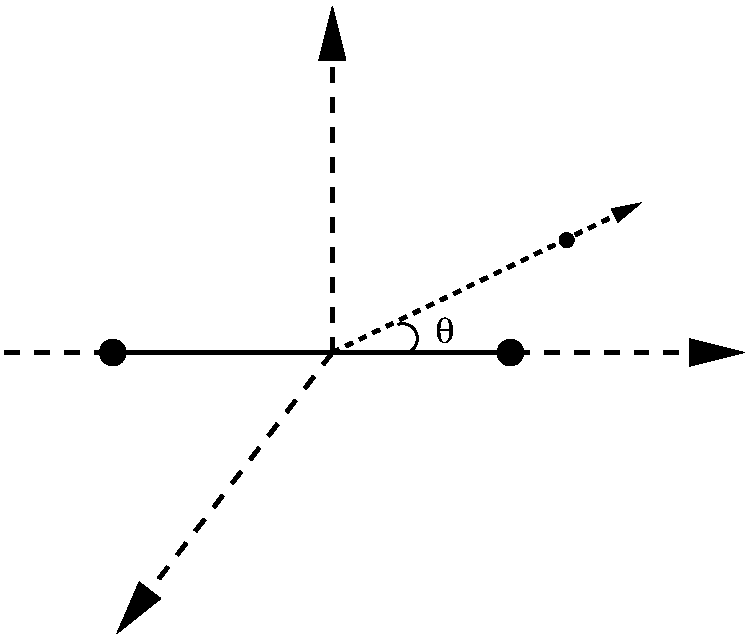
\includegraphics[scale=0.5]{sce.pdf}
%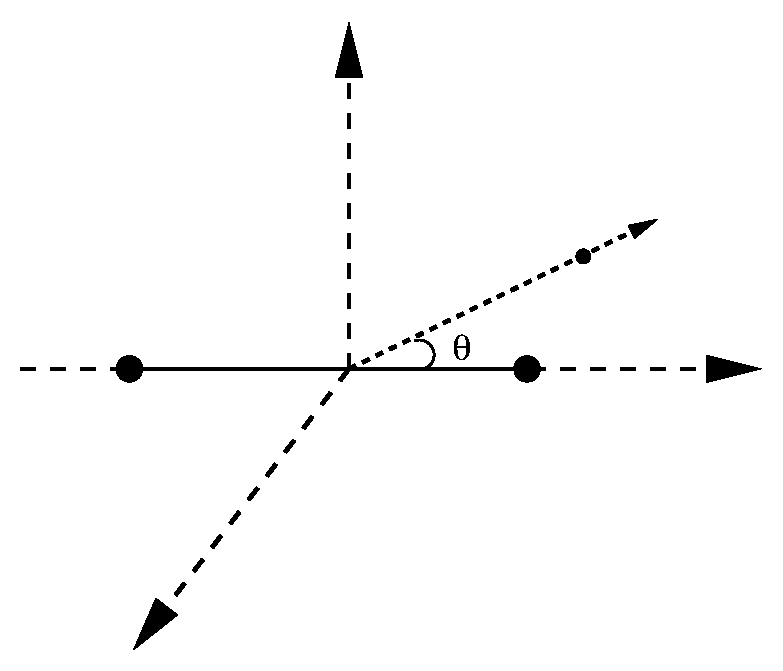
\includegraphics[scale=.5]{sce.eps}
\end{center}

Everything is referred to the origin of coordinate chosed as the center
of mass. Thus, for example, we expand the static potential energy
\Eq{vstel} as
\begin{equation}
  \label{eq:vstels}
\vstrel=\sum_{\lambda=0}^\infty\vls(r_{N+1})P_\lambda(\cos\theta_{N+1})  
\end{equation}
where for $\DIH$ targets only $\lambda$ = even appear.

\subsection{The Static Potential}
\label{sec:static-potential}
We've discussed the evaluation of $\vls$ in considerable detail in the
PhD thesis for a $\DIH$ molecule --- in particular, for CO$_2$
\footnote{see Michael A. Morrision's thesis}. Summarizing, we choose to
work from the charge density $\rho_\gamma(\ver)$ of the target, which is
defined for state $\gamma$ as
\begin{equation}
  \label{eq:den}
  \rho_\gamma(\ver) = \int\ewf\ewe\,\rd 1\cdots\,\rd (N-1)\sum\sigma_N
\end{equation}
Note that $\rho(\ver) = \rho(\ver,\Ra)$ since $\ew_\gamma$ depends
parametrically on the nuclear geometry. In terms of the spatial orbitals
$\owa(\ver)$ of \Eq{ew} and \Eq{sw}, we get
\begin{equation}
  \label{eq:dena}
\rho(\ver) = \sum_{j=1}^{N_{occ}}N_j|\ow_j(\ver)|^2
\end{equation}
where $N_j$ = occupation number of $j^{th}$ occupied spatial orbital.
Clearly, this makes sense only for a single configuation wavefunction of
the form of \Eq{ew}. $N_{occ}$ = number of occupied spatial orbitals.

We expand $\rho(\ver) = \rho(r,\theta)$ in Legendre polynomials,
obtaining
\begin{equation}
  \label{eq:denl}
  \rho(r,\theta) = \sum_{\lambda=0}^{\infty}a_\lambda(r)P_\lambda(\cos\theta)
\end{equation}
where
\begin{equation}
  \label{eq:alam}
  a_\lambda(r) = \dfrac{2\lambda+1}{2}
                 \int_0^\pi\rho(r,\theta)P_\lambda(\cos\theta)\sin\theta\,\rd\theta
\end{equation}
Again, only even-$\lambda$ coefficients contribute for $\DIH$ systems in
\Eq{denl}.

Each $\vls$ can be written
\begin{equation}
  \label{eq:vsts}
  \vls(r) = \vln(r) + \vle(r)
\end{equation}
where $\vln(r)$ arises form the $e$-nuclear interaction terms in $\Vint$
and $\vle$ from the $e$-$e$ term.

The nuclear term is easily evaluated. For example, for a homonuclear
diatomic target, we get 
\begin{equation}
  \label{eq:vlamn}
  \vln(r) = -2\Za\dfrac{\rho_{<}{}^{\lambda}}{\rho_{>}{}^{\lambda+1}}
\end{equation}
where $\Za$ is the nuclear charge on one of the centers and 
\begin{equation}
  \label{eq:rmR}
  \rho_{\substack{< \\ >}} = \substack{\min \\ \max}\Big\{r,\oneover{2}R\Big\}
\end{equation}
with $R$ the internuclear separation. For a triatiomic $\DIH$ molecule
with charge $Z_\beta$ at the origin, we get instead
\begin{equation}
  \label{eq:vlamnt}
  \vln(r) = -\dfrac{Z_\beta}{r}\delta_{\lambda 0}
            -2\Za\dfrac{\rho_{<}{}^{\lambda}}{\rho_{>}{}^{\lambda+1}}
\end{equation}

The evaluation of the electronic term is mere arduous, but left to the
similar expansion
\begin{equation}
  \label{eq:vlame}
  \vle(r) =
  \dfrac{4\pi}{2\lambda+1}\int_0^{\infty}a_\lambda(r')
  \dfrac{r_{<}{}^{\lambda}}{r_{>}{}^{\lambda+1}}r'{}^2\,\rd r'
\end{equation}
where
\begin{equation}
  \label{eq:rmr}
  r_{\substack{< \\ >}} = \substack{\min \\ \max}\big\{r,r'\big\}
\end{equation}
and $a_\lambda(r)$ comes from the expansion of \Eq{denl} and \Eq{alam}.

\subsection{The Coupled Equation for Elastic Scattering}
\label{sec:coupl-equat-elast}
We shall expand the scattering function $\sofnel$ in single-center
partial waves as
\begin{equation}
  \label{eq:sofnel}
  \sofnel = \oneover{r_{N+1}}\sum_{\ell'=0}^{\infty}\sum_{m'}\srfn\sshfn
\end{equation}
The approach is the usual one --- shove \Eq{sofnel} into \Eq{essc},
multiplied by $\sshfnb$ and $\int\rd\hat{r}_{N+1}$, viz.,
\begin{equation}
  \label{eq:essca}
    \begin{split}
    &\left[-\oneover{2}\lap_{N+1}+\vstrel-\oneover{2}k^2\right]
    \oneover{r_{N+1}}\sum_{\ell'm'}\srfn\sshfn \\
    =&-N\matrixelement{\ewc\swgb}
                     {\oneover{\rln}}
                     {\ewaa\sum_{\ell'm'}\oneover{r_1}\srfna\sshfna\swgc}
  \end{split}
\end{equation}

This can be written as
\begin{equation}
  \label{eq:esscb}
  \begin{split}
    &\left[\lap_{N+1}+k^2\right]\sofnel-2\vstrel\sofnel \\
    =&2N\matrixelement{\ewc\swgb}
                     {\oneover{\rln}}
                     {\ewaa\scfael}
  \end{split}
\end{equation}

If the exchange term were zero, we know what comes out of this, viz.,
\begin{equation}
  \label{eq:esscc}
  \left[\dfrac{\rd^2}{\rd
      r_{N+1}{}^2}-\dfrac{\ell'(\ell'+1)}{r_{N+1}{}^2}+k^2\right]\srfn
=2\sum_{\ell''}\vstlm(r_{N+1})\srfnb
\end{equation}
with
\begin{equation}
  \label{eq:mvst}
  \vstlm(r) = (-1)^{m'}\sqrt{(2\ell'+1)(2\ell''+1)}
                        \sum_{\lambda}\oneover{2\lambda+1}\vls(r)
                        \CG{\ell'\ell''\lambda;00}\CG{\ell'\ell''\lambda;-m',m'}
\end{equation}
with $\lambda$ = even for $\DIH$. Alas, the exchange term is NOT zero!

Using what we know, we can reduce \Eq{essca} [after $\otimes$
$\int\sshfnb\,\rd\hat{r}_{N+1}$ and interchange $\ell'$ and $\ell''$] to
\begin{equation}
  \label{eq:esscd}
    \begin{split}
    &\left[-\oneover{2}\dfrac{\rd^2}{\rd
        r_{N+1}{}^2}+\dfrac{\ell'(\ell'+1)}{2r_{N+1}{}^2}-\oneover{2}k^2\right]\srfn 
      + \sum_{\ell''}\vstlm(r_{N+1})\srfnb \\
   = &-r_{N+1}N\sum_{\ell''}\int\sshfnc \\
     & \matrixelement{\ewc\swgb}{\oneover{\rln}}
                     {\ewaa\left[\oneover{r_1}\srfnc\sshfnd\swgc\right]}\,\rd\hat{r}_{N+1}
  \end{split}
\end{equation}
and we must do something with the right side of \Eq{esscd}. [Note that
the integration is over $\rd 1\cdots\,\rd N\,\rd\hat{r}_{N+1}\sum\sigma_{N+1}$.]

We must resort to our formula \Eq{ew} for the molecular target
electronic wavefunctions,
\begin{equation}
  \label{eq:ewi}
  \ewt=\oneover{\sqrt{N!}}
  \sum_{\abpi}\LC_{\abpi}\sowai(1)\sowbi(2)\cdots\sowpi(N)
\end{equation}
where we've added a subscript $i$, which we'll need later.

\subsection{Structure of the Exchange Kernel: Reduction to $e$-H$_2$}
\label{sec:struct-exch-kern}
Before proceeding for this, se should note that we can write \Eq{esscd}
as
\begin{equation}
  \label{eq:essce}
    \begin{split}
    &\left[-\oneover{2}\dfrac{\rd^2}{\rd
        r_{N+1}{}^2}+\dfrac{\ell'(\ell'+1)}{2r_{N+1}{}^2}-\oneover{2}k^2\right]\srfn 
      + \sum_{\ell''}\vstlm(r_{N+1})\srfnb \\
   = &\sum_{\ell''}\int_0^{\infty}\Kex\srfnc\,\rd r_1
  \end{split}
\end{equation}
where
\begin{equation}
  \label{eq:kex}
  \begin{split}
  \Kex = &
  -N\dfrac{r_{N+1}}{r_1}\int\sshfnc\ewd\swgd\oneover{\rln}\ewaa \\ 
  &\sshfnd\swgc\,\rd\hat{r}_1\sum\sigma_1\,\rd 2\cdots\,\rd
  N\,\rd\hat{r}_{N+1}\sum\sigma_{N+1}
 \end{split}
\end{equation}
is the exchange kernel. For H$_2$ target, this reduces to 
\begin{equation}
  \label{eq:kexh}
  \begin{split}
  \Kexh = &
  -2\dfrac{r_3}{r_1}\int\sshfnh\ewh\swgh\oneover{\rlh}\ewah \\ 
  &\sshfnd\swgc\,\rd\hat{r}_1\sum\sigma_1\,\rd 2\,\rd\hat{r}_3\sum\sigma_3
 \end{split}
\end{equation}
where
\begin{equation}
  \label{eq:ewah}
  \ewah \equiv \ew(\ver_1,\ver_2;R)\tswh
\end{equation}

For the $^1\Sigma_g^+$ of H$_2$, the spin function is
\begin{equation}
  \label{eq:tswh}
  \tswh = \oneover{\sqrt{2}}[\alpha(1)\beta(2)-\beta(1)\alpha(2)]
\end{equation}
Here $\ew(\ver_1,\ver_2;R)$ is the spatial molecular target
function. Hence we have
\begin{equation}
  \label{eq:kexha}
  \begin{split}
  \Kexh = &
  -2\dfrac{r_3}{r_1}\int\sshfnh\ewhs\oneover{\rlh}\ewahs \\ 
  &\sshfnd\,\rd\hat{r}_1\,\rd\ver_2\,\rd\hat{r}_3
   \braket{\tsw(\sigma_1\sigma_2\sigma_3)|\tsw(\sigma_2\sigma_3\sigma_1)}
 \end{split}
\end{equation}
where the system spin function (3-electrons) is
\begin{equation}
  \label{eq:tsws}
  \tsw(\sigma_i\sigma_j\sigma_k) \equiv \oneover{\sqrt{2}}
  [\alpha(i)\beta(j)-\beta(i)\alpha(j)]\sww(k)
\end{equation}
and $\sww(k)$ is either $\alpha(k)$ or $\beta(k)$.

The matrix element
\begin{equation*}
\begin{split}
  \braket{\tsw(\sigma_1\sigma_2\sigma_3)|\tsw(\sigma_2\sigma_3\sigma_1)}
  = & 
  \sum_{1,2,3}\oneover{\sqrt{2}}[\alpha^*(1)\beta^*(2)-\beta^*(1)\alpha^*(2)]\sw^*(3) \\
  & \times \oneover{\sqrt{2}}[\alpha(2)\beta(3)-\beta(2)\alpha(3)]\sw(1) \\
  = &
  \oneover{2}\sum_{1,3}\alpha^*(1)\beta(3)\sw^*(3)\sw(1)\sum_2\beta^*(2)\alpha(2) \\
  - &
  \oneover{2}\sum_{1,3}\beta^*(1)\beta(3)\sw^*(3)\sw(1)\sum_2\alpha^*(2)\alpha(2) \\
  - &
  \oneover{2}\sum_{1,3}\alpha^*(1)\alpha(3)\sw^*(3)\sw(1)\sum_2\beta^*(2)\beta(2) \\
  + &
  \oneover{2}\sum_{1,3}\beta^*(1)\alpha(3)\sw^*(3)\sw(1)\sum_2\alpha^*(2)\beta(2) \\
\end{split}
\end{equation*}
And we have
\begin{equation*}
\begin{split}
  \sum_i\alpha^*(i)\alpha(i) = 1 \\
  \sum_i\beta^*(i)\beta(i) = 1 \\
  \sum_i\alpha^*(i)\beta(i) = 0 \\
  \sum_i\beta^*(i)\alpha(i) = 0 
\end{split}
\end{equation*}
So,
\begin{equation*}
\begin{split}
  \braket{\tsw(\sigma_1\sigma_2\sigma_3)|\tsw(\sigma_2\sigma_3\sigma_1)}
  = &
  - \oneover{2}\sum_{1,3}\beta^*(1)\beta(3)\sw^*(3)\sw(1) \\
  & - \oneover{2}\sum_{1,3}\alpha^*(1)\alpha(3)\sw^*(3)\sw(1)
\end{split}
\end{equation*}
Whether $\sw$ is $\alpha$ or $\beta$, we have
\begin{equation}
  \braket{\tsw(\sigma_1\sigma_2\sigma_3)|\tsw(\sigma_2\sigma_3\sigma_1)}
 = -\oneover{2}
\end{equation}
for doublet composite state $+$ singlet ground state, our current
example. We therefore see that our SE equations reduce to the results we
obtained earlier for elastic $e$-H$_2$, viz., we have
\begin{equation}
  \label{eq:essch}
    \begin{split}
    &\left[-\dfrac{\rd^2}{\rd r_3{}^2}+\dfrac{\ell'(\ell'+1)}{r_3{}^2}-k^2\right]\srfh 
      + 2\sum_{\ell''}\vstlm(r_3)\srfhb \\
   = &2\sum_{\ell''}\int_0^{\infty}\Kexh\srfhc\,\rd r_1
  \end{split}
\end{equation}
where
\begin{equation}
  \label{eq:kexhb}
  \Kexh = 
  \dfrac{r_3}{r_1}\int\sshfnh\ewhs\oneover{\rlh}\ewahs
  \sshfnd\,\rd\hat{r}_1\,\rd\ver_2\,\rd\hat{r}_3
\end{equation}
and $\ell_0$ denotes initial channel.

\subsection{General Exchange Kernel}
\label{sec:gener-exch-kern}
Now, let's call the exchange term [Right side of \Eq{esscd}] $-\I$,
viz.,
\begin{equation}
  \label{eq:Iex}
  \begin{split}
  -\I \equiv & r_{N+1}N\sum_{\ell''}\int\sshfnc \\
     & \matrixelement{\ewc\swgb}{\oneover{\rln}}
                     {\ewaa\left[\oneover{r_1}\srfnd\sshfnd\swgc\right]}\,\rd\hat{r}_{N+1} 
 \end{split}
\end{equation}
Note: drop $(\gamma)$ from $\srfnc$ here.

The first step will be to write $\I$ in terms of spin orbital using
\Eq{ewi}, as threatened earlier, we have for the $\ell''^{\underline{th}}$
term in $\I$,
\begin{multline}
  \label{eq:Iexll}
    \I^{(\ell'')} =
    r_{N+1}\dfrac{N}{N!}\int\sshfnc
     \left[\sum_i\LC_i\sowaib(1)\cdots\sowpib(N)\right]\swgd\oneover{\rln}\\
     \left[\sum_j\LC_j\sowaj(N+1)\sowbj(2)\cdots\sowpj(N)\right] \\
     \oneover{r_1}\srfnd\sshfnd\swgc\,\rd 1\cdots\,\rd N\,\rd\hat{r}_{N+1}\sum\sigma_{N+1}
\end{multline}
where $\LC_i\equiv\LC_{\abpi}$ and $\sum_i=\sum_{\abpi}$.

Clearly, 
\begin{equation}
  \label{eq:Iexa}
  \I = (-1)^{N}\sum_{\ell''} \I^{(\ell'')}
\end{equation}
since we have used 
\begin{equation*}
  \begin{split}
    \ew(2,3,4,\cdots,N,N+1;\Ra) & = -\ew(N+1,3,4,\cdots,N,2;\Ra) \\
                                & = +\ew(N+1,2,4,\cdots,N,3;\Ra) \\
                                & = -\ew(N+1,2,3,\cdots,N,4;\Ra) \\
                                & = (-1)^{i+1}\ew(N+1,2,4,\cdots,N,i;\Ra) \\
                                & = (-1)^{N-1+1}\ew(N+1,2,4,\cdots,N,N-1;\Ra) \\
                                & = (-1)^{N+1}\ew(N+1,2,4,\cdots,N-1,N;\Ra)
  \end{split}
\end{equation*}

Therefore \Eq{Iexll} is ``simply''
\begin{equation}
  \label{eq:Iexlla}
  \begin{split}
    \I^{(\ell'')} = r_{N+1}\dfrac{N}{N!}\sum_i\sum_j\LC_i\LC_j 
           & \int\sshfnc\swgd\sowaj(N+1)\sum\sigma_{N+1} \\
   \otimes & \int\sowbib(2)\sowbjb(2)\,\rd 2\cdots\int\sowpib(N)\sowpj(N)\,\rd N \\
   \otimes & \int\sowaib(1)\oneover{\rln}\left[\oneover{r_1}\srfnd\sshfnd\swgc\right]\,\rd 1\,\rd\hat{r}_{N+1}
  \end{split}
\end{equation}

Let' not worry about the orthonormality integral on the second line at
present. Instead, we'll work on 
\begin{equation}
  \label{eq:Iexllb}
  \begin{split}
  \bar{\J}_{ij}^{(\ell'')} & \equiv
  \int\sshfnc\swgd\sowaj(N+1) \\
  &\times\int\sowaib(1)\oneover{\rln}\left[\oneover{r_1}\srfnd\sshfnd\right]\swgc\,\rd 1\,\rd\hat{r}_{N+1}\sum\sigma_{N+1} 
  \end{split}
\end{equation}
From \Eq{sw} and the orthogonality of the spin wavefunction, the spin
integrations give $\delta_{m_s}(\alpha_j,N+1)\delta_{m_s}(\alpha_i,N+1)$
and the remaining radial $\int$ is
\begin{equation}
  \label{eq:Iexllc}
  \J_{ij}^{(\ell'')} =
  \int\sshfnc\owaj(\vrnone)\owaib(\ver_1)\oneover{\rln}\left[\oneover{r_1}\srfnd\sshfnd\right]\,\rd\ver_1\,\rd\hat{r}_{N+1}
\end{equation}

Now, as usual we expand
\begin{equation}
  \label{eq:rijexp}
  \oneover{\rln} = \sum_{\lambda=0}^{\infty} 
                   \dfrac{r_<{}^\lambda}{r_>{}^{\lambda+1}}
                   P_\lambda(\cos\angle(\vrnone,\ver_1))
\end{equation}
where
\begin{equation}
% \label{eq:2}
   r_{\substack{< \\ >}} = \substack{\min \\ \max}\big\{r_1,r_{N+1}\big\}
\end{equation}
or (from (4.28) in \cite{MER1957})
\begin{equation}
  \label{eq:rexp}
  \oneover{\rln} =
  \sum_{\lambda=0}^{\infty}\left(\dfrac{4\pi}{2\lambda+1}\right)
  \dfrac{r_<{}^\lambda}{r_>{}^{\lambda+1}}\sum_{\mu=-\lambda}^{+\lambda}
  \sshfne\sshfnf
\end{equation}
by the addition theorem of spherical harmonics. Therefore we have for
\Eq{Iexllc}
\begin{equation}
  \label{eq:Iexlld}
  \begin{split}
  \J_{ij}^{(\ell'')} = \sum_{\lambda\mu}\left(\dfrac{4\pi}{2\lambda+1}\right)
  & \int\sshfnc\owaj(\vrnone)\owaib(\ver_1)\dfrac{r_<{}^\lambda}{r_>{}^{\lambda+1}}\sshfne\sshfnf \\
  & \otimes\left[\oneover{r_1}\srfnd\sshfnd\right]\,\rd\ver_1\,\rd\hat{r}_{N+1}
  \end{split}
\end{equation}

To proceed further in the reduction of $\J_{ij}^{(\ell'')}$, we must
expand the molecular orbitals in single-center radial functions as
\begin{equation}
  \label{eq:moexp}
  \owa(\ver)=\oneover{r}\sum_{\orwsub}\orwa\sshorwa
\end{equation}
and we note again aximal symmetry, hence no $\sum_{m_\orwsupa}$ in
\Eq{moexp}

We'll re-introduce the sum over $\ell''$ from \Eq{Iex} and consider the
integral $\J_{ij} = \sum_{\ell''}\J_{ij}^{(\ell'')}$, i.e.,
\begin{equation}
  \label{eq:Iexb}
  \begin{split}
  \J_{ij} \equiv \sum_{\ell''}\sum_{\lambda\mu}\left(\dfrac{4\pi}{2\lambda+1}\right)
  & \int\sshfnc\owaj(\vrnone)\owaib(\ver_1)\dfrac{r_<{}^\lambda}{r_>{}^{\lambda+1}}\sshfne\sshfnf \\
  & \otimes\left[\oneover{r_1}\srfnd\sshfnd\right]\,\rd\ver_1\,\rd\hat{r}_{N+1}
  \end{split}
\end{equation}

Before we begin, the integral we're trying to evaluate, \Eq{Iex}, is
\begin{equation}
  \label{eq:Iexba}
  \I' =
  (-1)^{N}r_{N+1}\dfrac{N}{N!}\sum_{ij}\LC_i\LC_j\J_{ij}\delta_{m_s}(\alpha_j,N+1)\delta_{m_s}(\alpha_i,N+1)
\end{equation}
$\otimes(\text{orthogonal integral})$, where orthogonal integral is
\begin{equation*}
  \int\sowbib(2)\sowbjb(2)\,\rd 2\cdots\int\sowpib(N)\sowpj(N)\,\rd N 
\end{equation*}

Now, substituting \Eq{moexp} into \Eq{Iexb}, we get
\begin{equation}
  \label{eq:Iexc}
  \begin{split}
  \J_{ij} = \sum_{\ell''}\sum_{\lambda\mu}\left(\dfrac{4\pi}{2\lambda+1}\right)
  & \int\sshfnc\left[\oneover{r_{N+1}}\sum_{\orwsub}\orwb\sshorwb\right] \\
  & \otimes\left[\oneover{r_1}\sum_{\orwsuba}\orwc\sshorwc\right]\dfrac{r_<{}^\lambda}{r_>{}^{\lambda+1}}\sshfne\sshfnf \\
  & \otimes\left[\oneover{r_1}\srfnd\sshfnd\right]\,\rd\ver_1\,\rd\hat{r}_{N+1}
  \end{split}
\end{equation}

Rearranging the spherical functions and note that $\rd\ver = r^2\rd
r\rd\hat{r}$, we have
\begin{equation}
  \label{eq:Iexd}
  \begin{split}
  \J_{ij} = \sum_{\ell''}\sum_{\orwsub\orwsuba}\sum_{\lambda\mu}
            & \left(\dfrac{4\pi}{2\lambda+1}\right)\oneover{r_{N+1}}\orwb \\
            & \otimes\int r_1{}^2\,\rd
               r_1\oneover{r_1{}^2}\orwc\srfnd\dfrac{r_<{}^\lambda}{r_>{}^{\lambda+1}} \\
            & \otimes\int\rd\hat{r}_{N+1}\sshfnc\sshorwb\sshfne \\
            & \otimes\int\rd\hat{r}_1\sshfnd\sshorwc\sshfnf
  \end{split}
\end{equation}

The angular integrals are easily evaluated from the ever-popular Rose's
formula (4.34) and (4.31) \cite{MER1957}
\begin{equation}
  \label{eq:shadd}
  \int\rd\Omega\,\ssh_{\ell_3}^{m_3\,*}\ssh_{\ell_2}^{m_2}\ssh_{\ell_1}^{m_1} = 
  \sqrt{\dfrac{(2\ell_1+1)(2\ell_2+1)}{4\pi(2\ell_3+1)}}\,\CG{\ell_1\ell_2\ell_3;m_1m_2m_3}\CG{\ell_1\ell_2\ell_3;000}
\end{equation}
and
\begin{equation}
  \label{eq:consh}
  \ssh_{\ell}^{m\,*} = (-1)^m\ssh_{\ell}^{-m}
\end{equation}

We have in \Eq{Iexd} two integrals of this type, i.e., 
\begin{equation}
  \label{eq:shadda}
  \begin{split}
  \int\rd\Omega\,\ssh_{\ell'}^{m'\,*}\ssh_{\orwsub}^{m_\orwsupb}\ssh_{\lambda}^{\mu}
  & =
  (-1)^{m'+m_{\orwsupb}}\int\rd\Omega\,\ssh_{\orwsub}^{-m_\orwsupb\,*}\ssh_{\lambda}^{\mu}\ssh_{\ell'}^{-m'} \\
  & = (-1)^{m'+m_\orwsupb}\sqrt{\dfrac{(2\ell'+1)(2\lambda+1)}{4\pi(2\orwsub+1)}}\CG{\ell'\lambda\orwsub;-m',\mu,-m_\orwsupb}\CG{\ell'\lambda\orwsub;000}
  \end{split}
\end{equation}
and
\begin{equation}
  \label{eq:shaddb}
  \begin{split}
  \int\rd\Omega\,\ssh_{\ell''}^{m'}\ssh_{\orwsub'}^{m_\orwsupc\,*}\ssh_{\lambda}^{\mu\,*}
  & =
  (-1)^{\mu}\int\rd\Omega\,\ssh_{\orwsub}^{m_\orwsupc\,*}\ssh_{\lambda}^{-\mu}\ssh_{\ell''}^{m'} \\
  & = (-1)^{\mu}\sqrt{\dfrac{(2\ell''+1)(2\lambda+1)}{4\pi(2\orwsub'+1)}}\CG{\ell''\lambda\orwsub';m',-\mu,m_\orwsupc}\CG{\ell''\lambda\orwsub';000}
  \end{split}
\end{equation}

From (3.5) in \cite{MER1957}, notice that \Eq{shadda}
\begin{equation*}
  -m'+\mu = -m_\orwsupb
\end{equation*}
and
\begin{equation*}
  m'-\mu = m_\orwsupc
\end{equation*}
or
\begin{align*}
m' - \mu = m_\orwsupb \\
m' - \mu = m_\orwsupc
\end{align*}
where we see that $m_\orwsupb = m_\orwsupc$. This important result
simplifies the exchange term by limiting the number of MO's that appear
in any given $i^{th}$ term. We can further use this to carry out
$\sum_{\mu}$ in \Eq{Iexd}. Doing so with
\begin{equation}
  \label{eq:muindex}
  \mu = m' - m_\orwsupc
\end{equation}
we have
\begin{equation}
  \label{eq:Iexe}
  \begin{split}
  \J_{ij} = \sum_{\ell''}\sum_{\orwsub\orwsuba}\sum_{\lambda}
            & \left(\dfrac{4\pi}{2\lambda+1}\right)\oneover{r_{N+1}}\orwb \\
            & \otimes\int\rd
               r_1\orwc\srfnd\dfrac{r_<{}^\lambda}{r_>{}^{\lambda+1}}\delta_{m_\orwsupa}(i,j) \\
            &
            \otimes(-1)^{m'+m_\orwsupc}\sqrt{\dfrac{(2\ell'+1)(2\lambda+1)}{4\pi(2\orwsub+1)}}\CG{\ell'\lambda\orwsub;-m',m'-m_\orwsupc}\CG{\ell'\lambda\orwsub;00} \\
            & \otimes(-1)^{m'-m_\orwsupc}\sqrt{\dfrac{(2\ell''+1)(2\lambda+1)}{4\pi(2\orwsub'+1)}}\CG{\ell''\lambda\orwsub';m',m_\orwsupc-m'}\CG{\ell''\lambda\orwsub';00}
  \end{split}
\end{equation}
or
\begin{equation}
  \label{eq:Iexf}
  \begin{split}
  \J_{ij} = \sum_{\ell''}\sum_{\orwsub}\sum_{\orwsuba}\sum_{\lambda}
            & \oneover{r_{N+1}}\orwb\delta_{m_\orwsupa}(i,j)\int\rd
               r_1\orwc\srfnd\dfrac{r_<{}^\lambda}{r_>{}^{\lambda+1}} \\
            & \otimes\sqrt{\dfrac{(2\ell'+1)(2\ell''+1)}{(2\orwsub+1)(2\ell'+1)}}\CG{\ell'\lambda\orwsub;-m',m'-m_\orwsupc}\CG{\ell''\lambda\orwsub';m',m_\orwsupc-m'} \\
            & \otimes\CG{\ell'\lambda\orwsub;00}\CG{\ell''\lambda\orwsub';00}
  \end{split}
\end{equation}

Let's define a constant
\begin{equation}
  \label{eq:gl}
  \begin{split}
  \glm \equiv &
  \sqrt{\dfrac{(2\ell'+1)(2\ell''+1)}{(2\orwsub+1)(2\ell'+1)}}\,\CG{\ell'\lambda\orwsub;-m',m'-m_\orwsupc} \\
            &\otimes\CG{\ell''\lambda\orwsub';m',m_\orwsupc-m'}\,\CG{\ell'\lambda\orwsub;00}\,\CG{\ell''\lambda\orwsub';00}
  \end{split}
\end{equation}
so that
\begin{equation}
  \label{eq:Iexg}
  \J_{ij} = \sum_{\orwsub\orwsuba\ell''}\sum_{\lambda}
            \oneover{r_{N+1}}\orwb\delta_{m_\orwsupa}(i,j)\int\rd
               r_1\orwc\srfnd\dfrac{r_<{}^\lambda}{r_>{}^{\lambda+1}}\,\glm
\end{equation}

Therefore the final desired integral of \Eq{Iex} is,
\begin{equation}
  \label{eq:Iexh}
  \begin{split}
    \I = (-1)^{N}r_{N+1}\dfrac{N}{N!}
    &\sum_{ij}\LC_i\LC_j\J_{ij}\delta_{m_s}(\alpha_j,N+1)\delta_{m_s}(\alpha_i,N+1) \\
    &\otimes\int\sowbib(2)\sowbj(2)\,\rd 2\cdots\int\sowpib(N)\sowpj(N)\,\rd N 
  \end{split}
\end{equation}

Because of the $\delta$-function conditions in \Eq{Iexg} and \Eq{Iexh},
together with $N$ is even for closed-shell molecule, $\I$ becomes
\begin{equation}
  \label{eq:Iexha}
  \begin{split}
    \I & = r_{N+1}\dfrac{N}{N!}
    \sum_{i}\LC_i\J_{ii}\delta_{m_s}(\alpha_i,N+1)\int\sowbib(2)\sowbi(2)\,\rd 2\cdots\int\sowpib(N)\sowpi(N)\,\rd N \\
       & = r_{N+1}\dfrac{N}{N!}
    (N-1)!\sum_{i=1}^{N}\J_{ii}\delta_{m_s}(\alpha_i,N+1)
  \end{split}
\end{equation}
Notice that the last sum index $i$ means summing from the first electron
orbital over the $N^{th}$ electron orbital.

Substituting \Eq{Iexg} into \Eq{Iexha}, we get
\begin{equation}
  \label{eq:Iexi}
  \I = \sum_{i}^{N}\sum_{\orwsub\orwsuba\ell''\lambda}
            \orwba\delta_{m_s}(\alpha_i,N+1)\glm\int\rd
               r_1\orwc\srfnd\dfrac{r_<{}^\lambda}{r_>{}^{\lambda+1}}
\end{equation}

Thus the coupled equations \Eq{esscd} become [we'll drop the $\alpha$
stuff --- call it $i$]
\begin{equation}
  \label{eq:esscf}
    \begin{split}
    &\left[-\oneover{2}\dfrac{\rd^2}{\rd
        r_{N+1}{}^2}+\dfrac{\ell'(\ell'+1)}{2r_{N+1}{}^2}-\oneover{2}k^2\right]\srfne
      + \sum_{\ell''}\vstlm(r_{N+1})\srfnf \\
   = &\sum_{i=1}^{N}\sum_{\orwsub\orwsuba\ell''\lambda}
      \orwbb\delta_{m_s}(i,N+1)\glma\int\rd
      r_1\orwca\srfhc\dfrac{r_<{}^\lambda}{r_>{}^{\lambda+1}}
  \end{split}
\end{equation}

Notice that we only get an exchange term from electrons with the same
spin as the scattering electron --- because of $\delta_{m_s}(i,N+1)$.
This is certinly reasonable (remember Hartree-Fock).

It is useful to modify our notation still further to clean up
\Eq{esscf}. Let $\ell_0$ denote the initial angular momentum. Alas, of
course, for closed-shell molecules, each spatial MO will contain one
electron with the same spin as that of the $(N+1)^{th}$ electron (we'll
treat $\pi_g(x)$ and $\pi_g(y)$ as different orbitals). Thus we have
\begin{equation}
  \label{eq:CEES}
  \begin{split}
    &\left[\dfrac{\rd^2}{\rd r_{N+1}{}^2}
      -\dfrac{\ell(\ell+1)}{r_{N+1}{}^2}+k^2\right]\srfng \\
    = & 2\sum_{\ell'}\left[\vstlma(r_{N+1})\srfnh - \int\rd
      r_1\,\KEX\srfni\right]
  \end{split}
\end{equation}
where (notice the sum index $i$ means summing from the lowest spatial
orbital to the highest occupied spatial orbital)
\begin{equation}
  \label{eq:KEX}
  \KEX = \sum_{i=1}^{N_{occ}}\sum_{\ell''\ell'''\lambda}
  \orwbc\orwcb\glmb\dfrac{r_<{}^\lambda}{r_>{}^{\lambda+1}}
\end{equation}
with
\begin{equation}
  \label{eq:glm}
  \begin{split}
  \glmb & = \sqrt{\dfrac{(2\ell+1)(2\ell'+1)}{(2\ell''+1)(2\ell'''+1)}}\,
  \CG{\ell\lambda\ell'';-m,m-m_i}\,\CG{\ell\lambda\ell'';00} \\
  & \otimes \CG{\ell'\lambda\ell''';m,m_i-m}\,\CG{\ell'\lambda\ell''';00}
  \end{split}
\end{equation}
and
\begin{equation}
  \label{eq:rlam}
  r_{\substack{< \\ >}} = \substack{\min \\ \max}\big\{r_1,r_{N+1}\big\}
\end{equation}

Notice that for N$_2$, for instance, with configuration X$^1\Sigma_g^+$:
\begin{equation*}
  1\sigma_g{}^2 2\sigma_g{}^2 3\sigma_g{}^2 1\sigma_u{}^2 1\sigma_u{}^2
  1\pi_u(x)^2 1\pi_u(y)^2
\end{equation*}
we have $N_{occ} = 7$.

There are some restrictions placed on the summmations in the exchange
kernel, i.e., $\gla$ does it:
\begin{subequations}
  \begin{align}
    \label{eq:glres}
    \ell + \lambda + \ell''  = \text{even} & \qquad (\lambda \geq 0) \\
    \ell' + \lambda + \ell''' = \text{even}& \\
    |\ell - \ell''| \leq \lambda  \leq \ell + \ell'' & \qquad
    [\Delta(\ell\lambda\ell'')]     \label{eq:glresc} \\
    |\ell' - \ell'''| \leq \lambda \leq \ell' + \ell'''& \qquad
    [\Delta(\ell'\lambda\ell''')] \label{eq:glresd}
  \end{align}
\end{subequations}
but this would help much! Recall that, e.g., $\orwbd$ is the expansion
coefficient of the $i^{th}$ molecular orbital corresponding to
$P_{\ell''}(\cos\theta)$ --- i.e., the $\ell''^{th}$ partial wave. Note
also that we can write the exchange kernel as
\begin{equation}
  \label{eq:KEXa}
  \KEX = \sum_{i=1}^{N_{occ}}\sum_{\ell''\ell'''}
  \orwbc\orwcb\sum_{\lambda}\glmb\dfrac{r_<{}^\lambda}{r_>{}^{\lambda+1}}
\end{equation}

It is certainly not hard to see from \Eq{KEX} why the number of exchange
kernel rapidly gets out of hand. For a given $\ell$ (e.g., $\ell = 0
\sim$ ``s-in'') we couple, say, one partial wave $\ell'$ on the right
hand side in the exchange term (we already know from painful experience
how many $\ell'$ are usually need in the static coupling term!). Then we
get a huge number of exchange term arising from the $\ell''\ell''$ and
$\lambda$, say, in $\Kexa$.

Of course, the static coupling matrix element in \Eq{mvst},
\begin{equation}
  \label{eq:mvsta}
  \vstlma(r_{N+1}) = (-1)^{m}\sqrt{(2\ell+1)(2\ell'+1)}
                        \sum_{\lambda}\oneover{2\lambda+1}\vls(r_{N+1})
                        \CG{\ell\ell'\lambda;00}\CG{\ell\ell'\lambda;-m,m}
\end{equation}

Parenthetically, we note that using the properties of the Clebesh-Gordon
coefficients (\cite{MER1957}-(3.17c)), we get
\begin{subequations}
  \begin{align}
%     \label{eq:3}
    \CG{\ell\ell'\lambda;-m,m} & =
      (-1)^{\ell'+m}\sqrt{\dfrac{2\lambda+1}{2\ell+1}}\,\CG{\ell'\lambda\ell;-m,0} \\
    \CG{\ell\ell'\lambda;00} & =
      (-1)^{\ell'}\sqrt{\dfrac{2\lambda+1}{2\ell+1}}\,\CG{\ell'\lambda\ell;00}
  \end{align}
\end{subequations}
where
\begin{equation}
  \label{eq:mvstb}
  \vstlma(r_{N+1}) = \sqrt{\dfrac{2\ell'+1}{2\ell+1}}
                        \sum_{\lambda}\vls(r_{N+1})
                        \,\CG{\ell'\lambda\ell;-m,0}\,\CG{\ell'\lambda\ell;00}
\end{equation}
or, using \cite{MER1957}-(3.16a),
\begin{equation}
  \label{eq:mvstc}
  \vstlma(r_{N+1}) = \sqrt{\dfrac{2\ell'+1}{2\ell+1}}
                        \sum_{\lambda}\vls(r_{N+1})
                        \,\CG{\ell'\lambda\ell;m,0}\,\CG{\ell'\lambda\ell;00}
\end{equation}
For $\DIH$ targets, only $\lambda = $ even contribute to $\sum_\lambda$
in \Eq{mvstc}.

\subsection{Example: $e$-H$_2$}
\label{sec:example:-e-h_2}
We have
\begin{equation}
  \label{eq:CEESh}
  \begin{split}
    &\left[\dfrac{\rd^2}{\rd r_{3}{}^2}
      -\dfrac{\ell(\ell+1)}{r_{3}{}^2}+k^2\right]\srfngh \\
    = & 2\sum_{\ell'}\left[\vstlma(r_{3})\srfnhh - \int\rd
      r_1\,\KEXh\srfni\right]
  \end{split}
\end{equation}
where
\begin{equation}
  \label{eq:KEXh}
  \KEXh = \sum_{\ell''\ell'''\lambda}
  \orwbch\orwcbh\glmbh\dfrac{r_<{}^\lambda}{r_>{}^{\lambda+1}}
\end{equation}
where we note that for H$_2$ there is only one spatial orbital ---
$\sigma_g$, so the $\sum_i$ vanishes; also, of course, $m(\sigma_g) =
0$.

We know from experience that about 3 partial waves is sufficient --- say
$s$, $d$, $g$ --- to coverage the static problem. Consider $\sigma$-wave
scattering ($m = 0$), i.e., $\Sigma_g$ symmetry $+ \Sigma_u$
\begin{enumerate}
\item $s$-wave ($\ell = 0$) $\Rightarrow$ always have $\lambda = \ell''$
  by \Eq{glresc}  \qquad [$\Sigma_g$]
  \begin{enumerate}
  \item Expand MO in 1 term (spherical only) $\Rightarrow \ell'' =
    \ell''' = 0$ $\Rightarrow \lambda = 0$ (by \Eq{glresc}) $\Rightarrow
    \ell' = 0$ (by \Eq{glresd})

    Exchange term in \Eq{CEESh} becomes
    \begin{equation*}
      -2\int\rd r_1\K^{(0)}(00|r_1r_3)\Y_{0\ell_0}^{(0)}
    \end{equation*}
    with
    \begin{equation*}
      \K^{(0)}(00|r_1r_3) =
      \orw_0^{\orwsuph}(r_3)\orw_0^{\orwsuph}(r_1)\g_0(0000;00)\oneover{r_1} 
    \end{equation*}
    One exchange term only.
  \item Expand MO in 2 terms: $\ell'' = 0, 2$; $\ell''' = 0, 2$ allowed
    and $\lambda = \ell''$ (by \Eq{glresc})

    Exchange kernel becomes ($\sum' \Rightarrow$ even only),
    \begin{equation*}
      \K^{(0)}(0\ell'|r_1r_3) ={\sum_{\ell''=0}^2}'{\sum_{\ell'''=0}^2}'
      \orw_{\ell''}^{\orwsuph}(r_3)\orw_{\ell'''}^{\orwsuph}(r_1)
      \g_{\ell''}(0\ell'\ell''\ell''';00)\dfrac{r_<{}^{\ell''}}{r_>{}^{\ell''+1}}
    \end{equation*}
    with $|\ell'-\ell'''| \leq \ell'' \leq \ell'+\ell'''|$

    Exchange term becomes
    \begin{equation*}
      -2\int\rd r_1\left[\K^{(0)}(00|r_1r_3)\Y_{0\ell_0}^{(0)}(r_1)
                        +\K^{(0)}(02|r_1r_3)\Y_{2\ell_0}^{(0)}(r_1)
                        +\K^{(0)}(04|r_1r_3)\Y_{4\ell_0}^{(0)}(r_1)\right]
    \end{equation*}
  \end{enumerate}
\item $p$-wave ($\ell = 1$) $\Rightarrow |1-\ell''| \leq \lambda \leq
  1+\ell''$ \qquad [$\Sigma_u$]
  \begin{enumerate}
  \item Expand MO in 1 term $\Rightarrow \ell''=\ell'''=0$ $\Rightarrow
    \lambda =1$ and $\ell'=1$

    Again only
    \begin{equation*}
      -2\int\rd r_1\K^{(0)}(11|r_1r_3)\Y_{1\ell_0}^{(0)}(r_1)
    \end{equation*}
    with
    \begin{equation*}
      \K^{(0)}(11|r_1r_3) =
      \orw_0^{\orwsuph}(r_3)\orw_0^{\orwsuph}(r_1)\g_1(1100;00)\dfrac{r_<}{r_>{}^2}
    \end{equation*}
  \item Expand MO in 2 terms: $\ell'' = 0, 2$; $\ell''' = 0, 2$ allowed
    and $|1-\ell''| \leq \lambda \leq 1+\ell''$ and $|\ell'-\ell'''|
    \leq \lambda \leq \ell'+\ell'''$

    Exchange term
    \begin{equation*}
      -2\int\rd r_1\left[\K^{(0)}(11|r_1r_3)\Y_{1\ell_0}^{(0)}(r_1)
                        +\K^{(0)}(13|r_1r_3)\Y_{3\ell_0}^{(0)}(r_1)
                        +\K^{(0)}(15|r_1r_3)\Y_{5\ell_0}^{(0)}(r_1)\right]
    \end{equation*}
  \end{enumerate}
\end{enumerate}

\subsection{The General Case: ``Simplification'' of the exchange term}
\label{sec:gener-case:-simpl}
Let's return to the case of an $N$ electron target with $N_{occ}$
spatial orbitals. Suppose an molecule has $\sigma$ and $\pi$ molecular
orbitals. We can write (no longer treating $\pi_x$ separately from
$\pi_y$) 
\begin{equation}
  \label{eq:KEXSP}
  \begin{split}
  \KEX & = \sum_{i=1}^{N_{occ}(\sigma)}\sum_{\ell''\ell'''\lambda}
  \orwbcs\orwcbs\glmbs\dfrac{r_<{}^\lambda}{r_>{}^{\lambda+1}} \\
       & + \sum_{i=1}^{N_{occ}(\pi)}\sum_{\ell''\ell'''\lambda}
  \orwbcp\orwcbp\glmbpa\dfrac{r_<{}^\lambda}{r_>{}^{\lambda+1}} \\
       & + \sum_{i=1}^{N_{occ}(\pi)}\sum_{\ell''\ell'''\lambda}
  \orwbcp\orwcbp\glmbpb\dfrac{r_<{}^\lambda}{r_>{}^{\lambda+1}} 
  \end{split}
\end{equation}

For the $\sigma$-orbital, we call
\begin{equation}
  \label{eq:Alm}
  \glmbs \equiv \Alm
\end{equation}
and for the $\pi$-orbital, we call
\begin{equation}
  \label{eq:Blm}
  \glmbpa + \glmbpb \equiv \Blm
\end{equation}

Thus we get (in this notation)
\begin{equation}
  \label{eq:KEXSPa}
  \begin{split}
  \KEX & = \sum_{i=1}^{N_{occ}(\sigma)}\sum_{\ell''\ell'''\lambda}
  \orwbcs\orwcbs\dfrac{r_<{}^\lambda}{r_>{}^{\lambda+1}}\Alm \\
       & + \sum_{i=1}^{N_{occ}(\pi)}\sum_{\ell''\ell'''\lambda}
  \orwbcp\orwcbp\dfrac{r_<{}^\lambda}{r_>{}^{\lambda+1}}\Blm
  \end{split}
\end{equation}
and the exchange term in the scattering equations becomes (call it $\I$)
\begin{equation}
  \label{eq:ET}
  \begin{split}
    \I \equiv & -2\sum_{\ell'}\int\rd r_1\,\KEX\srfni \\
      = & -2\sum_{\ell'}\int\rd r_1\left[\sum_{i=1}^{N_{occ}(\sigma)}\sum_{\ell''\ell'''\lambda}
  \orwbcs\orwcbs\dfrac{r_<{}^\lambda}{r_>{}^{\lambda+1}}\Alm\right. \\
       & + \left.\sum_{i=1}^{N_{occ}(\pi)}\sum_{\ell''\ell'''\lambda}
  \orwbcp\orwcbp\dfrac{r_<{}^\lambda}{r_>{}^{\lambda+1}}\Blm\right]\srfni \\
      = & -2\sum_{\ell'}\left[\sum_{i=1}^{N_{occ}(\sigma)}\sum_{\ell''\ell'''\lambda}
  \orwbcs\Alm\int_0^{\infty}\rd r_1\orwcbs\srfni\dfrac{r_<{}^\lambda}{r_>{}^{\lambda+1}}\right. \\
       & + \left.\sum_{i=1}^{N_{occ}(\pi)}\sum_{\ell''\ell'''\lambda}
  \orwbcp\Blm\int_0^{\infty}\rd r_1\orwcbp\srfni\dfrac{r_<{}^\lambda}{r_>{}^{\lambda+1}}\right]
  \end{split}
\end{equation}

If we define
\begin{equation}
  \label{eq:Zlam}
  \Zlam[f_1,f_2;r'] \equiv \int_0^{\infty}\rd
  rf_1(r)f_2(r)\dfrac{r_<{}^\lambda}{r_>{}^{\lambda+1}} 
\end{equation}
with
\begin{equation*}
    r_{\substack{< \\ >}} = \substack{\min \\ \max}\big\{r,r'\big\}
\end{equation*}

Expanding, we have
\begin{equation}
  \label{eq:Zlama}
  \Zlam[f_1,f_2;r'] = \oneover{r'^{\lambda+1}}\int_0^{r'}\rd
  r\left[r^{\lambda}f_1(r)f_2(r)\right] + r'^{\lambda}\int_{r'}^{\infty}\rd
  r\left[\oneover{r^{\lambda+1}}f_1(r)f_2(r)\right] 
\end{equation}

Then the exchange term becomes
\begin{equation}
  \label{eq:ETa}
    \begin{split}
    \I = & -2\sum_{\ell'}\left\{\sum_{i=1}^{N_{occ}(\sigma)}\sum_{\ell''\ell'''\lambda}
  \orwbcs\Alm\Zlam\left[\orwcbs\srfni;r_{N+1}\right]\right. \\
       & + \left.\sum_{i=1}^{N_{occ}(\pi)}\sum_{\ell''\ell'''\lambda}
  \orwbcp\Blm\Zlam\left[\orwcbp\srfni;r_{N+1}\right]\right\}
  \end{split}
\end{equation}

[For N$_2$, $N_{occ}(\sigma) = 5$, $N_{occ}(\pi) = 1$.]

Then the coupled equations \Eq{CEES} become
\begin{equation}
  \label{eq:CEESN}
  \begin{split}
    &\left[\dfrac{\rd^2}{\rd r_{N+1}{}^2}
      -\dfrac{\ell(\ell+1)}{r_{N+1}{}^2}+k^2\right]\srfng \\
    = & 2\sum_{\ell'}\vstlma(r_{N+1})\srfnh  \\
    - & 2\sum_{i=1}^{N_{occ}(\sigma)}\sum_{\ell'\ell''\ell'''\lambda}
        \Alm\orwbcs\Zlam\left[\orwcbs\srfni;r_{N+1}\right] \\
    - & 2\sum_{i=1}^{N_{occ}(\pi)}\sum_{\ell'\ell''\ell'''\lambda}
        \Blm\orwbcp\Zlam\left[\orwcbp\srfni;r_{N+1}\right]
  \end{split}
\end{equation}

\subsection{Summary}
\label{sec:summary}
In a truly heroic effort, we have derived the coupled scattering
equations for electron-molecule scattering in the body-fixed frame of
reference including exchange. We make the Born-Oppenheimer approximation
on the target and do not allow for electronic excitation by electron
impact. Restricting ourselves to closed-shell targets. We obtain the
coupled equations of \Eq{sc} for the scattering functions $\sofn$ for
vibrational excitation. 

The reduction to radial equations has been carried out for elastic
scattering in a 1-center coordinate system. We find that an exchange
term appears for each target electron which has the same spin as that of
the $(N+1)^{th}$ electron. We get \Eq{CEES}-\Eq{glm} for the radial
scattering function $\srfng$. The static matrix element is given by
\Eq{mvst} or, equivalently, \Eq{mvsta}. The exchange kernel is given by
\Eq{KEX} subject to the restrictions of \Eq{glres}. The functions
$\orw_{\ell}^{(i)}$ appearing in \Eq{KEX} are the single-center
expansion terms of the $i^{th}$ spatial MO --- see \Eq{moexp}. Finally,
we showed that the coupled equation can be written in the magically more
useful form \Eq{CEESN}.

\section{The Coupled Equation for Vibrationally Inelastic Scattering}
\label{sec:coupl-equat-vibr}
Although we have derived the scattering equation \Eq{CEES}, we have to
keep in mind that \Eq{CEES} is derived from the original \Eq{essc},
which treats the system as a rigid rotor and does not allow vibrational
excitation. So \Eq{CEES} is only available for elastic scattering.

If we want to consider the vibrational excitation, we'll go back to
\Eq{sc}. From \Eq{mw}, we notice that the difference between \Eq{CEES}
and \Eq{sc} is that we omit the nuclear vibrational function
$\vw_{\nlvg}^{vib}(\Ra)$ and the sum index $v_{\gamma''}$. Checking
carefully from \Eq{essc} to \Eq{CEES}, we can find that although we
treated the target in fixed nuclei and derived the static coupling
matrix element \Eq{mvstb} and the exchange kernel \Eq{KEX}, we can
easily add the nuclear vibrational function and do not effect the
exchange kernel. 

So, we can write the coupled equation for vibrationally inelastic
scattering as (replacing $v_{\gamma'}$ to $v'$ for simplicity)
\begin{equation}
  \label{eq:vcea}
  \begin{split}
    &\left[\dfrac{\rd^2}{\rd r_{N+1}{}^2}
      -\dfrac{\ell(\ell+1)}{r_{N+1}{}^2}+k_v{}^2\right]\srfvl(r_{N+1}) \\
    = & 2\sum_{v'\ell'}\left[\vstvlm(r_{N+1})\srfvla(r_{N+1})-\int\rd r_1\,\vKEX\srfvla(r_1)\right]
  \end{split}
\end{equation}
with
\begin{equation}
  \label{eq:cvst}
  \vstvlm(r_{N+1}) = \int\vw_{v}{}^*(\Ra)\vstlma(r_{N+1};\Ra)\vw_{v'}(\Ra)\,\rd\Ra
\end{equation}
and
\begin{equation}
  \label{eq:ckex}
  \vKEX = \int\vw_{v}{}^*(\Ra)\KEXc\vw_{v'}(\Ra)\,\rd\Ra\
\end{equation}

\subsection{Polarization Potential}
\label{sec:polar-potent}
Recalling that we specialize to the case where no electronic excitation
is allowed (in page~\pageref{com:state}). i.e., we have neglected all of
the higher discrete and continuum electronic states. However, the
presence of a charged scattering projectile will cause the target
molecular system to distort. This distortion or ``polarization'' of the
target density gives rise an additional contribution to the system. This
additional contribution to the system energy is known as a
\textit{polariztion potential}. This difference in the system energy
when calculated with a distorting charge present and in its absence can
be taken into account by adding a polariztion term
$\hat{\mathcal{V}}_{pol}$.

Unfortunately, the polarization term is a non-local one. So exact
polarization term is hardly calculated. If we take a model potential,
which is supposed to be only subject to the spatial coordinates of the
scattering electron --- $V_{pol}(\vrnone)$, and expand it in Legendre
polynomials as \Eq{vstels}, we have
\begin{equation}
  \label{eq:vpolel}
  V_{pol}(\vrnone;\Ra) = \sum_{\lambda=0}^\infty\vlp(r_{N+1};\Ra)P_\lambda(\cos\theta_{N+1})  
\end{equation}

So, we can define
\begin{equation}
  \label{eq:vstpol}
  \vlsp(r_{N+1};\Ra) = \vls(r_{N+1};\Ra) + \vlp(r_{N+1};\Ra)
\end{equation}
and \Eq{mvstc} becomes
\begin{equation}
  \label{eq:mvsp}
  \vstlma(r_{N+1};\Ra) = \sqrt{\dfrac{2\ell'+1}{2\ell+1}}
                        \sum_{\lambda}\vlsp(r_{N+1};\Ra)
                        \,\CG{\ell'\lambda\ell;m,0}\,\CG{\ell'\lambda\ell;00}
\end{equation}

Substituting \Eq{mvsp} into \Eq{cvst}, we get
\begin{equation}
  \label{eq:cvsp}
  \begin{split}
  \vstvlm(r_{N+1}) = &
  \sum_{\lambda}\left[\int\vw_{v}{}^*(\Ra)\vlsp(r_{N+1};\Ra)\vw_{v'}(\Ra)\,\rd\Ra\right] \\
  &\times\sqrt{\dfrac{2\ell'+1}{2\ell+1}}\CG{\ell'\lambda\ell;m,0}\,\CG{\ell'\lambda\ell;00}
  \end{split}
\end{equation}

If we define
\begin{equation}
  \label{eq:glam}
  p_{\lambda}(\ell\ell';m) = \sqrt{\dfrac{2\ell'+1}{2\ell+1}}\CG{\ell'\lambda\ell;m,0}\,\CG{\ell'\lambda\ell;00}
\end{equation}
and
\begin{equation}
  \label{eq:clsp}
  \omega_{v,v'}^{\lambda}(r_{N+1}) = \int\vw_{v}{}^*(\Ra)\vlsp(r_{N+1};\Ra)\vw_{v'}(\Ra)\,\rd\Ra
\end{equation}
\Eq{cvsp} becomes 
\begin{equation}
  \label{eq:cvspa}
  \vstvlm(r_{N+1}) = \sum_{\lambda}p_{\lambda}(\ell\ell';m)\omega_{v,v'}^{\lambda}(r_{N+1})
\end{equation}

\subsection{Arrangement of the Coupled Equation for Vibrationally Inelastic Scattering}
\label{sec:arrang-coupl-equat}
In most references, the index $m$ is usually replaced by $\Lambda$ for
electron scattering from diatomic molecules in body-fixed frame. So we
rewrite all the coupled equations as
\begin{equation}
  \label{eq:vce}
  \begin{split}
    &\left[\dfrac{\rd^2}{\rd r_{N+1}{}^2}
      -\dfrac{\ell(\ell+1)}{r_{N+1}{}^2}+k_v{}^2\right]\vrsf(r_{N+1}) \\
    = & 2\sum_{v'\ell'}\left[\vcvst(r_{N+1})\vrsfa(r_{N+1})-\int\rd r_1\,\vckex\vrsfa(r_1)\right]
  \end{split}
\end{equation}
where the coupled local potential is
\begin{equation}
  \label{eq:vcsp}
  \begin{split}
  \vcvst(r_{N+1}) = &
  \sum_{\lambda}\left[\int\vw_{v}{}^*(\Ra)\vlsp(r_{N+1};\Ra)\vw_{v'}(\Ra)\,\rd\Ra\right] \\
  &\times\sqrt{\dfrac{2\ell'+1}{2\ell+1}}\CG{\ell'\lambda\ell;\Lambda,0}\,\CG{\ell'\lambda\ell;00}
  \end{split}
\end{equation}
and the coupled exchange term is
\begin{equation}
  \label{eq:vckex}
  \vckex = \int\vw_{v}{}^*(\Ra)\vckexk\vw_{v'}(\Ra)\,\rd\Ra\
\end{equation}
in which the exchange kernel is
\begin{equation}
  \label{eq:KEXb}
  \vckexk = \sum_{i=1}^{N_{occ}}\sum_{\ell''\ell'''}
  \orwbcn\orwcbn\sum_{\lambda}\glmbn\dfrac{r_<{}^\lambda}{r_>{}^{\lambda+1}}
\end{equation}
with
\begin{equation}
  \label{eq:glmbn}
  \begin{split}
  \glmbn & = \sqrt{\dfrac{(2\ell+1)(2\ell'+1)}{(2\ell''+1)(2\ell'''+1)}}\,
  \CG{\ell\lambda\ell'';-\Lambda,\Lambda-m_i}\,\CG{\ell\lambda\ell'';00} \\
  & \otimes \CG{\ell'\lambda\ell''';\Lambda,m_i-\Lambda}\,\CG{\ell'\lambda\ell''';00}
  \end{split}
\end{equation}

If the isolated molecule only contains $\sigma$ and $\pi$ orbitals, both
of which are fully occupied, we have (from \Eq{KEXSPa}),
\begin{equation}
  \label{eq:KEXc}
  \begin{split}
  \vckexk & = \sum_{i=1}^{N_{occ}(\sigma)}\sum_{\ell''\ell'''\lambda}
  \orwbcsn\orwcbsn\dfrac{r_<{}^\lambda}{r_>{}^{\lambda+1}}\Ala \\
       & + \sum_{i=1}^{N_{occ}(\pi)}\sum_{\ell''\ell'''\lambda}
  \orwbcpn\orwcbpn\dfrac{r_<{}^\lambda}{r_>{}^{\lambda+1}}\Bla
  \end{split}
\end{equation}
where
\begin{equation}
  \label{eq:Ala}
  \Ala = \glas
\end{equation}
and 
\begin{equation}
  \label{eq:Bla}
  \Bla = \glabpa + \glabpb
\end{equation}
We must note that in \Eq{KEXc} \textsl{there is only one $\pi$ orbital
  for N$_2$} since $\pi(x)$ and $\pi(y)$ are summed up through \Eq{Bla}.

\subsection{Comments on the Vibrationally Inelastic Scattering Equationns}
\label{sec:comm-vibr-inel}
Using \Eq{vce}-\Eq{Bla}, we could calculate the scattering function
numerically. Before doing that, we have to understand the physical
meaning of every variable and function.
\begin{itemize}
\item $r_{N+1}$: the radial coordinate of the scattering electron
\item $\ell_0$ and $\ell$: the initial and highest orbital angular
  momentum number of the scattering electron
\item $\Lambda$: the eigenvalue of $\ell_z$, projection of $\vec{\ell}$
  along the $\hat{e}_z$ (the internuclear axis for a diatomic molecule,
  $\hat{e}_z = R$). 

  Since $\hat{\mathcal{H}}_m^{(r)} = 0$ in the FNO
  (Fixed-Nuclear-Orientation) approximation, $\hat{\ell}_z$, the
  projection of the operator $\hat{L}$ onto the internuclear axis $R$
  (denoted by the symbol $\Lambda$) is a \textit{constant-of-motion}.
  Thus scattering quantities such as the K-matrix and T-matrix are
  diagonal in $\Lambda$. This leads to considerable simplifications, so
  much so, that various values of $\Lambda$ have been assigned spedific
  names. For homonuclear diatomic molecule, the inversion symmetry $g$
  or $u$ is specified. The first four symmetry designations are
  \begin{subequations}
    \begin{align}
      \label{eq:Lambda}
      \Sigma_g \quad & \Lambda = 0 \quad \ell = 0, 2, 4, \ldots \\
      \Sigma_u \quad & \Lambda = 0 \quad \ell = 1, 3, 5, \ldots \\
      \Pi_u    \quad & \Lambda = 1 \quad \ell = 1, 3, 5, \ldots \\
      \Pi_g    \quad & \Lambda = 1 \quad \ell = 2, 4, 6, \ldots 
    \end{align}
  \end{subequations}

  From \Eq{vce}, we only get T-matrix
  $\mathrm{T}_{v\ell,v_0\ell_0}^{\Lambda}$, through which the cross
  sections are calculated,
  \begin{subequations}
    \begin{align}
      \label{eq:ICS}
      \sigma_{v_0\rightarrow v}^{\Lambda} & =
      \dfrac{\pi}{k_0}\sum_{\ell,\ell_0}
      |\mathrm{T}_{v\ell,v_0\ell_0}^{\Lambda}|^2 \\
      \sigma_{v_0\rightarrow v} & = \sum_{\Lambda}\sigma_{v_0\rightarrow v}^{\Lambda}
    \end{align}
  \end{subequations}
\item $k_v$: energy of the scattering electron
  \begin{equation}
    \label{eq:5}
    k_v{}^2 = 2(E-\epsilon_v)
  \end{equation}
  where $\epsilon_v$ is the molecular energy at the $v^{th}$
  vibrational state and $E$ is the total energy of the scattering
  system.
\item $\ell'$: summing index, the same meaning as $\ell$

  For each $\Lambda$, we should specify a maximum of $\ell$ ---
  $\ell_{\max}$. Thus $\ell_0$, $\ell$ and $\ell'$ range from
  $\ell_{\min}$ and $\ell_{\max}$. For example, if we specify
  $\ell_{\max} = 9$ for $\Pi_u$, $\ell_0$, $\ell$ and $\ell'$ could be
  $1$, $3$, $5$, $7$ and $9$.
\item $v_0$ and $v$: the initial and final vibrational state of the target.
\item $v'$: summing index. More vibrational states are included to
  calculate the vibrational scattering. For example, for $v_0 = 0
  \Rightarrow v = 1$ of $e$-N$_2$, 15 vibrational states are needed. So
  the sum over $v'$ is from 0 to 14.
\item $\lambda$: summing index. $\lambda$ is the index of Legendre
  polynomials to expand $1/r_{1,N+1}$. $\lambda$ is from 0 to
  $\lambda_{\max}$. However, from \Eq{glres}, $\ell+\lambda+\ell''$ should be even, the initial $\lambda$ is \texttt{mod}($\ell+\ell''$,2) and the step is also 2 for homonuclear molecule.
\item $i$: summing index, the number of the molecular orbitals.
\item $\ell''$ and $\ell'''$: summing index, the number of spherical
  harmonic functions to expand the molecular orbitals from \Eq{moexp}
  and \Eq{CEES}.  
  \begin{subequations}
    \begin{align}
      \label{eq:lambda}
      \sigma_g \quad &  \ell''(\ell''') = 0, 2, 4, \ldots \\
      \sigma_u \quad &  \ell''(\ell''') = 1, 3, 5, \ldots \\
      \pi_u    \quad &  \ell''(\ell''') = 1, 3, 5, \ldots
    \end{align}
  \end{subequations}
\item $m_i$: the parity of the molecular orbital.
  \begin{subequations}
    \begin{align}
      \label{eq:moparity}
      \sigma \quad &  m_i = 0 \\
      \pi    \quad &  m_i = 1
    \end{align}
  \end{subequations}
\end{itemize}
\bibliography{SCIENCE_REFERENCES.bib}

\end{document}
